\subsection{Калибровка точного времени (Fine time calibration)}\label{section:FTcalib}

Пример таблицы калибровки точного времени, полученной на данных лабораторных тестов, представлен в виде графика на \figref{fig:TypicalCalibTable}. По оси абсцисс откладывается значение счётчика точного времени, а по оси ординат --- значение точного времени в наносекундах. Вид графика не зависит от того, по каким данным он был построен, так как он определяется архитектурой время-цифрового преобразователя. Обратим внимание, что в показанном примере в диапазоне значений десятибитного счетчика точного времени интервалу равному периоду грубого счетчика, т.е. 5~нс, соответствуют отсчеты от~30 до~520. Точные границы интервала определяются значениями задержек на элементах цифровой линии задержки. Эти величины индивидуальны и зависят от флуктуаций технологического процесса.

С целью понимания особенностей работы счётчиков точного времени, каждая таблица калибровки точного времени была аппроксимирована кусочно-линейной функцией. На \figref{fig:CalibTableMinusFit} показан пример разности значений функции калибровки точного времени и линейной функции. Видно, что отклонения не превышают 60~пс.

% Макросы для получения этих картинок лежат в Data_analysis_repo/threshold_scan_2/
\begin{figure}[H]
\centering
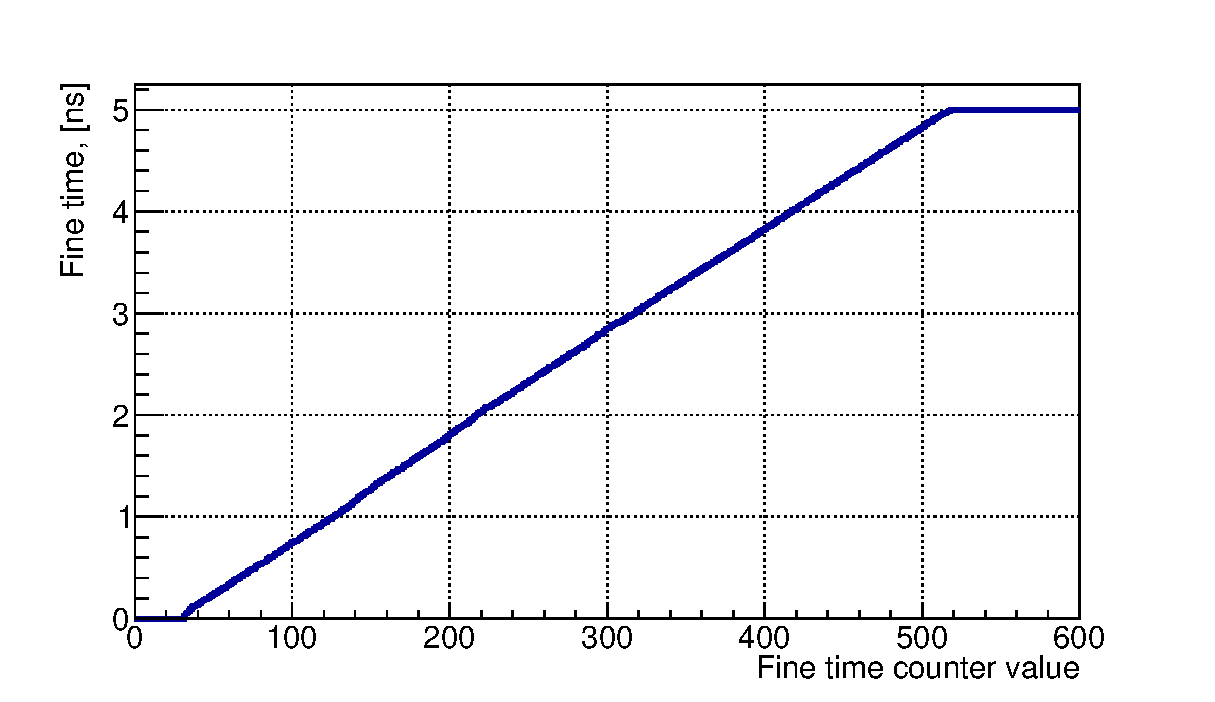
\includegraphics[width=1.0\textwidth]{pictures/17_CalTable_0010_01_feb2017.eps}
\caption{Пример калибровочной кривой.}
\label{fig:TypicalCalibTable}
\end{figure}

% Макросы для получения этих картинок лежат в Data_analysis_repo/threshold_scan_2/
\begin{figure}[H]
\centering
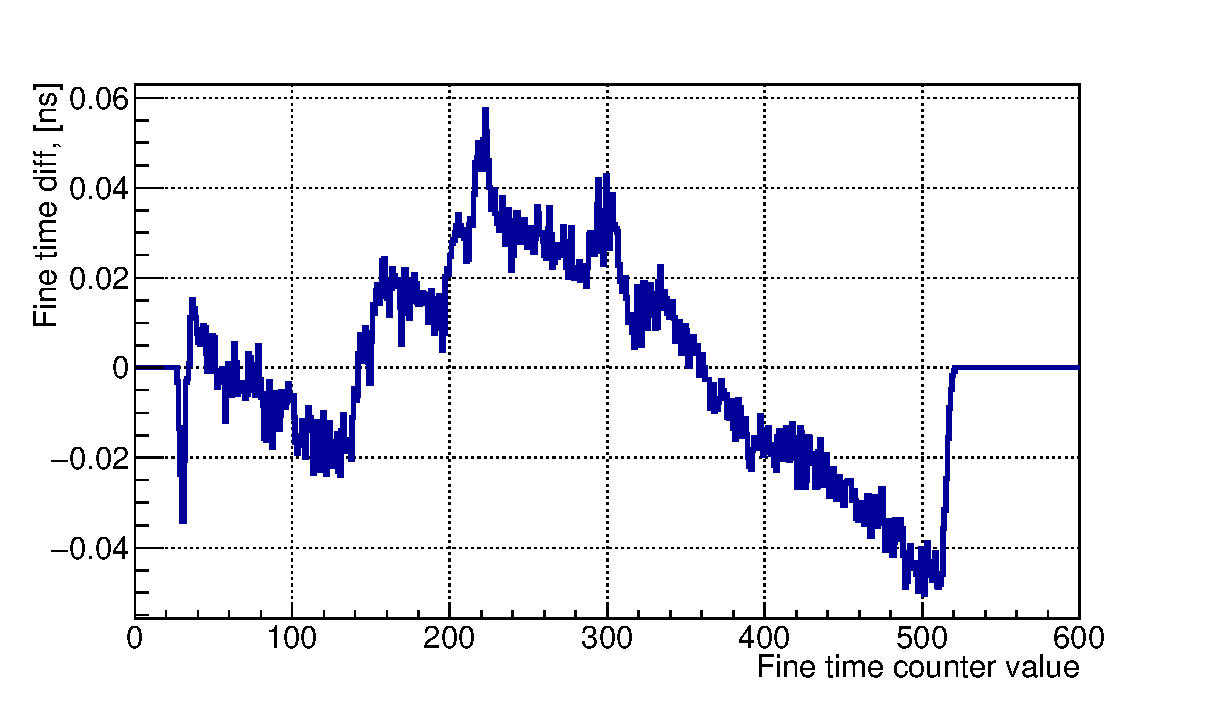
\includegraphics[width=1.0\textwidth]{pictures/18_CalTableMinusFit_0010_01_feb2017.eps}
\caption{Отклонение калибровочной кривой от линейной функции.}
\label{fig:CalibTableMinusFit}
\end{figure}

Каждая аппроксимирующая кусочно-линейная функция состоит из трёх отрезков и может быть однозначно описана двумя координатами изломов, которые приблизительно соответствуют двум крайним рабочим значениям счётчика точного времени. Параметры линейных функций для всех каналов отображены на двумерной диаграмме на \figref{fig:ABmap}. Видно, что хотя параметры и локализованы в двух областях, распределение достаточно компактное.

Для оценки влияния калибровки на точность регистрации временных отметок можно исследовать как одновременные фронты на разных каналах ВЦП, так и длительности прямоугольных импульсов во входных каналах, полученных с помощью высокоточного генератора прямоугольных импульсов. В работе~\cite{PEPAN} показано, что предельное временное разрешение в обоих случаях одинаково. Ниже мы используем второй подход.

В процедуре калибровки для каждого канала была выполнена замена точной калибровочной таблицы сначала индивидуальной линейной функцией данного канала, а потом общей функцией, усредненной по всем каналам (параметры этой функции показаны на \figref{fig:ABmap} сплошным квадратом). Полученные распределения измеренной ширины импульса в исследуемом входном канале показаны на \figref{fig:FourToT}. Там же показаны результаты без калибровки.

Видно, что использование точной калибровочной таблицы необходимо для достижения предельного разрешения ВЦП. Ширина распределения разностей временных отметок в двух независимо флуктуирующих каналах ВЦП составляет 30~пс~(FWHM), что соответствует временному разрешению 21~пс. Использование индивидуальной линейной функции приводит к увеличению ширины на полувысоте до 70~пс, а усреднённой --- до 90~пс в наиболее неблагоприятных каналах. Отметим, что использование усредненной линейной функции для калибровки устраняет двухпиковую форму, характерную для распределения без калибровки, но в некоторых случаях приводит при этом к увеличению ширины.
%Про первый просто написать, что он двугорбый - см. рисунок.
%Теперь в "наиболее неблагоприятных каналах" при глобальной псевдокалибровке тоже двугорбое распределение, которому не совсем честно приписывать 90 пс FWHM.

Таким образом, при невозможности выполнить калибровку точного времени, например, из-за недостаточного массива данных, предоставленных для анализа, в условиях нашей задачи, когда характерное временное разрешение составляет несколько сотен пикосекунд, возможно применение усредненной линейной функции без заметного снижения точности.

Использование усреднённой калибровки может быть особенно полезно при измерении разности временных отметок, полученных ВЦП различного типа, поскольку тогда, в отличие от нашего случая, не происходит сокращения начального сдвига кусочно-линейной функции относительно нуля регистра точного времени.

% Макросы для получения этих картинок лежат в Analysis_Sep2016/WLS_off/calibration_files/
\begin{figure}[H]
\centering
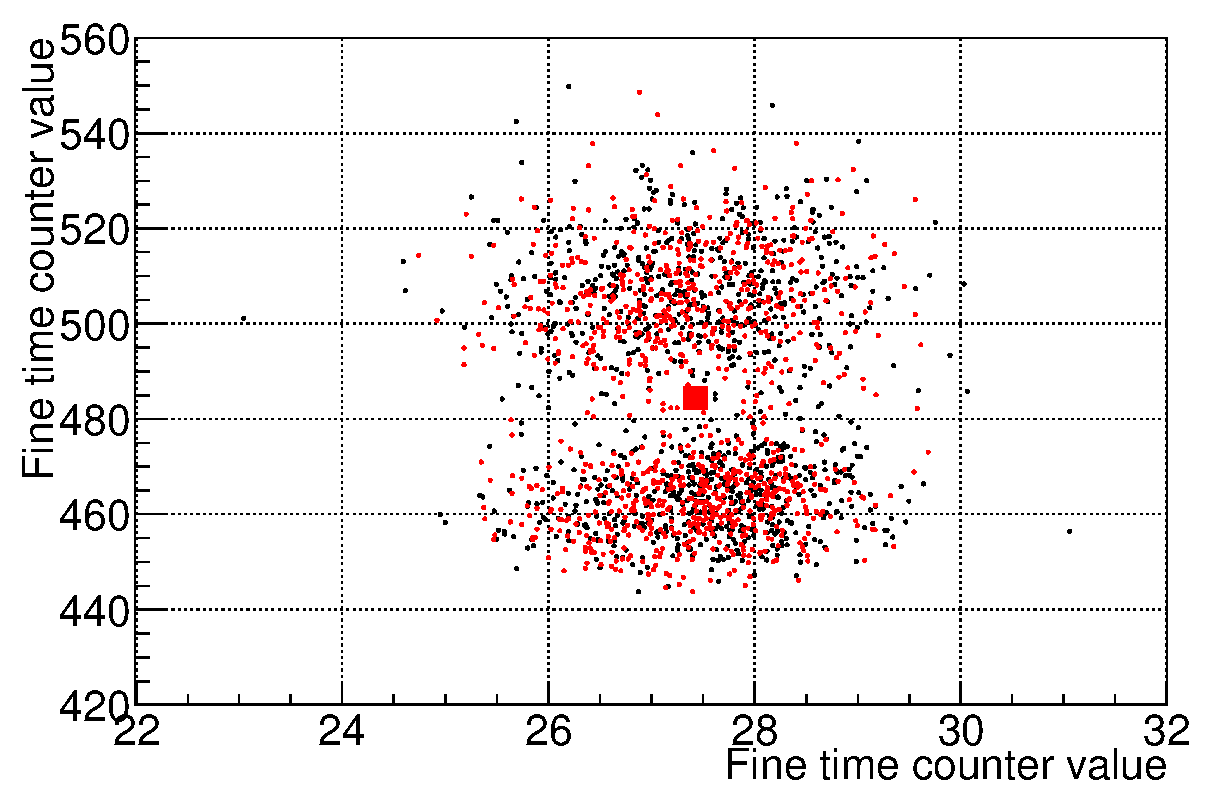
\includegraphics[width=1.0\textwidth]{pictures/19_ABmap.eps}
\caption{Распределение координат точек излома аппроксимирующих кусочно-линейных функций. Квадратом отмечено среднее значение, используемое для усредненной линейной функции.}
% для большого набора каналов по данным с пучковых тестов
\label{fig:ABmap}
\end{figure}

% Макросы для получения этих картинок лежат в Data_analysis_repo/directTDC/
\begin{figure}[H]
\centering
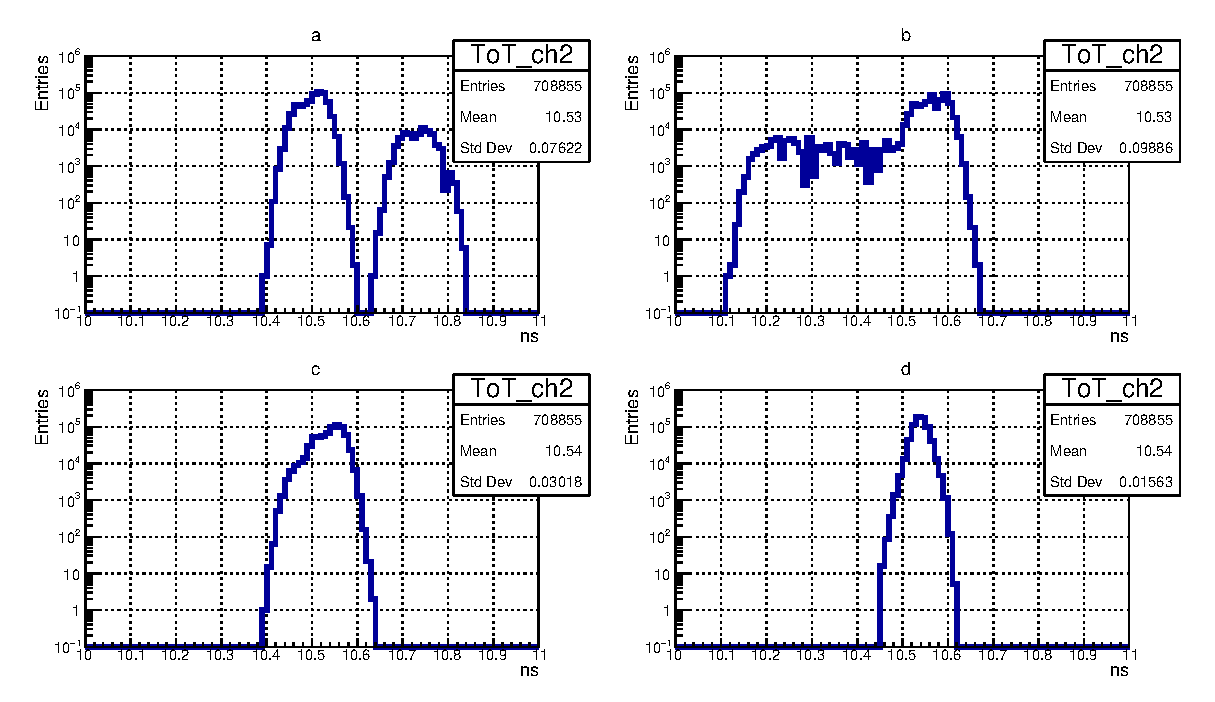
\includegraphics[width=1.0\textwidth]{pictures/20_ToT_ch2.eps}
\caption{Результаты измерения ширины импульса от генератора в случае: (a) без калибровки точного времени; (b) с применением усреднённой калибровочной фукнции; (c) с применением индивидуальной линейной калибровочной функции; (d) с применением полноценной калибровочной функции.}
\label{fig:FourToT}
\end{figure}

Приведённые выше таблицы калибровки были построены по массиву данных, содержащихся в семи файлах. Каждый файл соответствует двум минутам измерений при частоте генератора 5~кГц, т. е. около 600~тысяч вспышек лазера. Таким образом, всего было 4.2~миллиона вспышек за  14~минут, а один файл составляет приблизительно 15\%~от полного набора данных. В каждом канале было зарегистрировано от~300 до~400~тысяч временных отметок, которые были использованы для выполнения калибровки. Для иллюстрации стабильности калибровки на \figref{fig:Stability} показана разность функций калибровки, построенных по всему массиву данных и функций, построенных на файлах, составляющих $ \approx $15\%~данных каждый, взятых в начале, середине и конце набора данных. Видно, что отклонения в основном не превышают 10~пс, однако имеются редкие выбросы до 20~пс.

\begin{figure}[H]
\centering
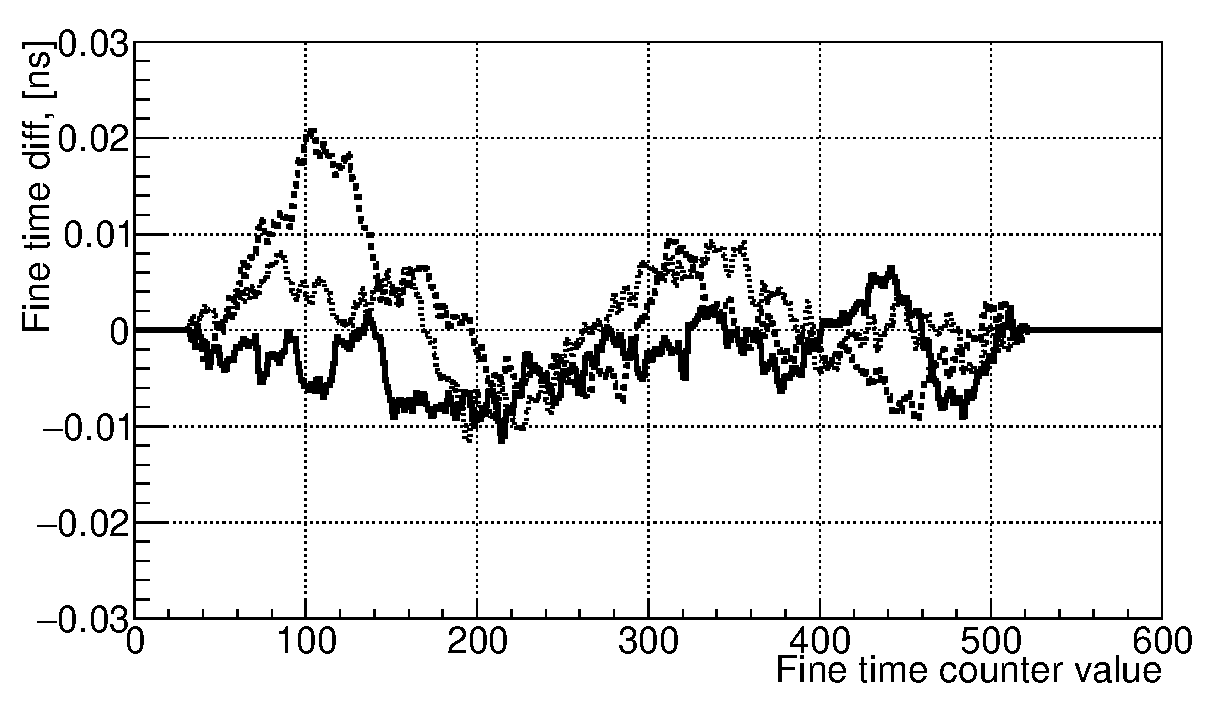
\includegraphics[width=1.0\textwidth]{pictures/21_calibrationStability_feb2017.eps}
\caption{Стабильность калибровок.}
\label{fig:Stability}
\end{figure}
